\documentclass{article}

\usepackage{float}
\usepackage{amsmath}
\usepackage{graphicx}
\usepackage{booktabs}

\title{Assignment of ET 4389}
\author{Volker Strobel}
\date{\today}

\begin{document}
\maketitle

I'm a guest student from the Radboud University. My TU Delft student
number is 4524187, my official start date at the TU Delft is March
2016, however, I have not received my login details yet. Therefore,
I've used my employee account (I'm also doing an internship here) for
this assignment.

\subsection*{1)}
$G$ is the network described in \texttt{7.txt}.

\begin{itemize}
  \item Number of nodes $N$: $379$ 
  \item Number of links $L$: $914$
  \item Link density $p$: $0.013$
  \item Average degree $E[D]$: $4.82$
  \item Degree variance $Var[D]$: $15.46$
\end{itemize}

\begin{figure}[H]
  \centering
  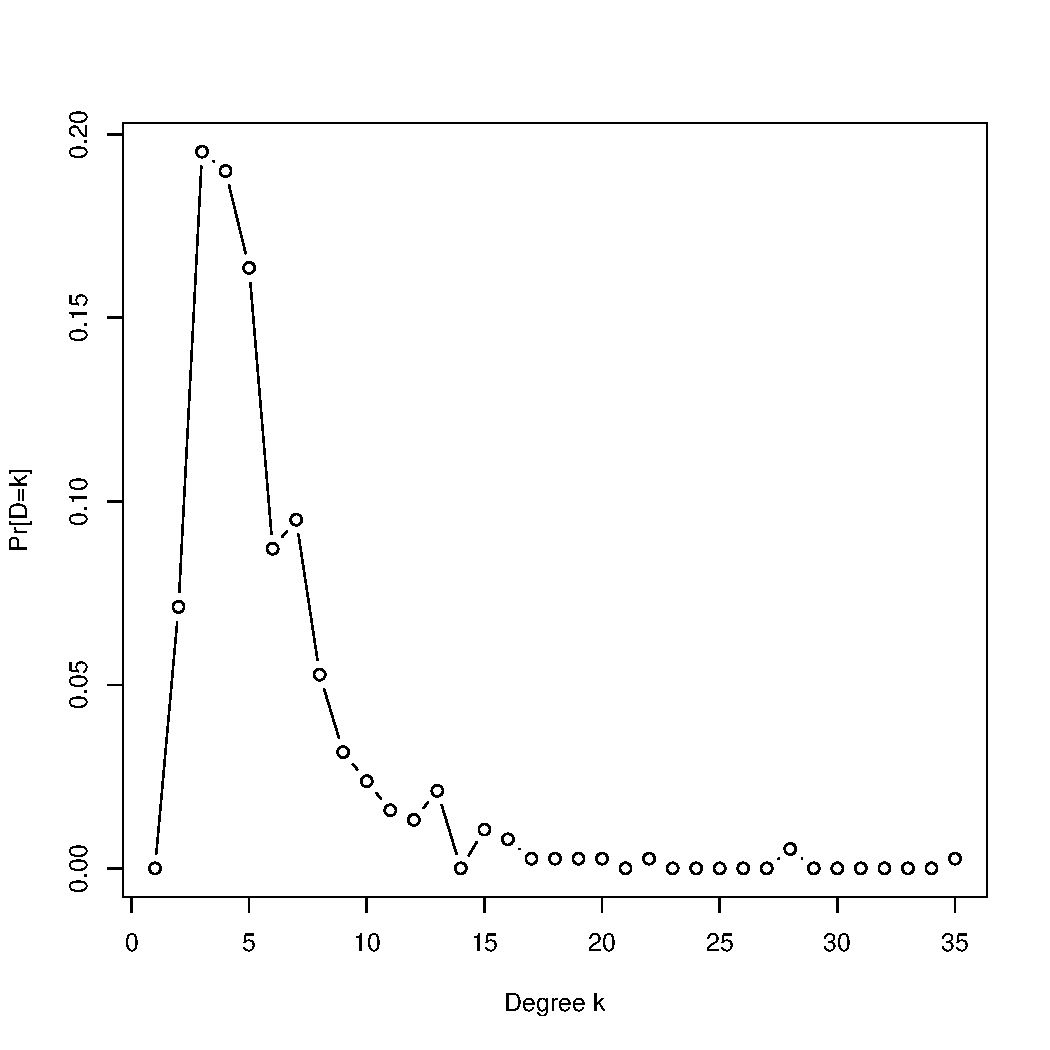
\includegraphics[width=0.7\textwidth]{degree_distribution}
  \caption{Degree distribution of Graph $G$}
\end{figure}

The degree distribution approximately follows a power law
distribution; however, the degrees 1 and 2 are underrepresented --
therefore, a lognormal distribution might be better suited. The
fitting curve for the power law distribution, with $\gamma = - 1.53$
is shown in Figure~\ref{fig:fitted-curve}.

\begin{figure}[H]
  \centering
  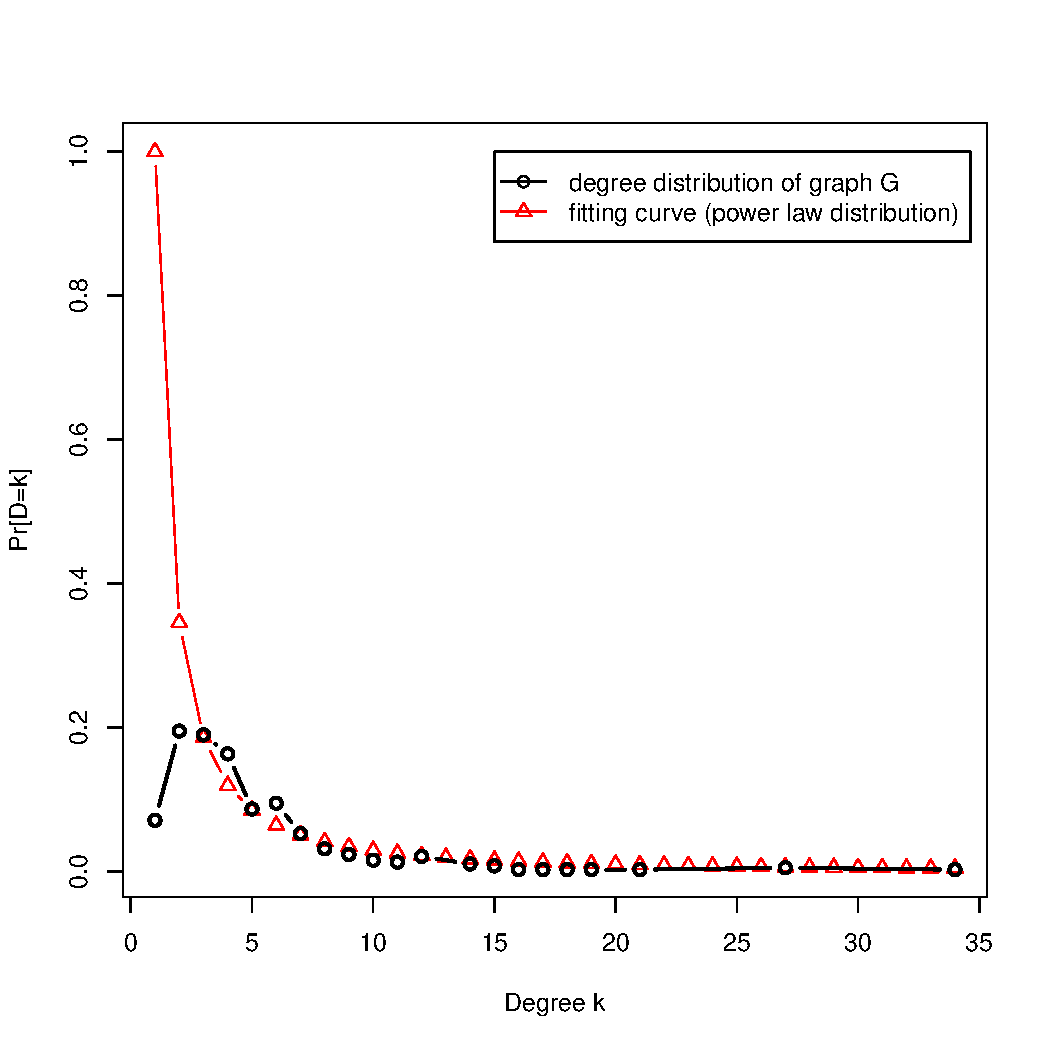
\includegraphics[width=0.7\textwidth]{fitted_curve}
  \caption{Fitting curve for graph $G$, with power exponent
    $\gamma = - 1.53$.}
  \label{fig:fitted-curve}
\end{figure}

\subsection*{2)}
The scale-free property strongly correlates with the network's
robustness to failure. It turns out that the major hubs are closely
followed by smaller ones. These smaller hubs, in turn, are followed by
other nodes with an even smaller degree and so on. This hierarchy
allows for a fault tolerant behavior. If failures occur at random and
the vast majority of nodes are those with small degree, the likelihood
that a hub would be affected is almost negligible. Even if a
hub-failure occurs, the network will generally not lose its
connectedness, due to the remaining hubs. On the other hand, if we
choose a few major hubs and take them out of the network, the network
is turned into a set of rather isolated graphs. Thus, hubs are both a
strength and a weakness of scale-free networks. These properties have
been studied analytically using percolation theory by Cohen et
al.[9][10] and by Callaway et al.[11]
\begin{itemize}
\item Degree correlation (assortativity) $\rho_D$: $-0.30$
\end{itemize}
\textbf{Physical meaning}:\\
Assortativity $\sim$ \emph{Birds of a feather flock together.}\\
Disassortativity $\sim$ \emph{Opposites attract.}

\vspace*{0.5em}
\noindent Networks, in which nodes with a high degree are likely
connected to other high-degree nodes are \emph{assortative}; networks
in which nodes with a low degree are likely connected to high-degree
nodes are \emph{disassortative}.

\subsection*{3)}

\begin{itemize}
  \item Clustering coefficient: $0.17$
\end{itemize}

\subsection*{4)}

\begin{itemize}
  \item Average hopcount $E[H]$: $3.75$
  \item Diameter $H_{max}$: $7$
\end{itemize}

\subsection*{5)}
\begin{itemize}
  \item Largest eigenvalue (spectral radius) $\lambda_1$: $7.44$
\end{itemize}
\subsection*{6)}

\begin{itemize}
\item Second smallest eigenvalue (algebraic connectivity) of the
  Laplacian matrix $\mu_{N-1}$: $0.40$
\end{itemize}

\subsection*{7)}
Now, we consider the network $G_N$, described in \texttt{NetScience.txt}.

\begin{itemize}
\item Number of nodes $N$: $379$
\item Number of links $L$: $914$
\item Link density $p$: $0.013$
\item Average degree $E[D]$: $4.82$
\item Degree variance $Var[D]$: $15.46$
\item Clustering coefficient $C$: $0.80$
\item Assortativity $\rho_D$: $-0.08$
\item Average hopcount $E[H]$: $6.04$
\item Spectral radius $\lambda_1$: $10.38$
\item Algebraic connectivity $\mu_{N-1}$: $0.015$
\item Diameter $H_{max}$: $17$
\end{itemize}

\subsection*{8)}

I am discussing the metrics in the sense of ``which network may allow
information to propagte to a larger fraction of the network'' an not,
for example, ``which network is better suited in case of attacks'' or
``which network might prevent the spread of a virus''.
\vspace*{0.5em}

\noindent\emph{Clustering coefficient $C$}. The clustering coefficient $C$
states how densely the neighbors of a node are connected. The physical
meaning in a communication network is, are my partners also connected
to each other. Here, $G_N$ performs much better
($C(G) = 0.17 < C(G_N) = 0.80$), and is therefore better suited, since
information can be sent on several channels. This makes the network
more robust in case of failures (e.g. node/link removal).

\vspace*{0.5em}
\noindent\emph{Average hopcount E[H]}. The average hopcount states the expected
length of the shortest path between two nodes. The physical meaning in
a communication network, this can be interpreted as the delay of the
network. The smaller the average hopcount, the smaller the delay, and
the faster messages can be sent between two partners. Since the
average hopcount of $H$ is $3.75$, messages can be send much faster
than in $G_N$ with a $E[H] = 6.04$.

\vspace*{0.5em}
\noindent\emph{Diameter $H_{max}$}. The diameter of the communication network
states how many edges a message needs to pass between two nodes in the
worst case. Since a smaller $H_{max}$ means faster communication in
the worst case, $G$ performs better ($H_{max}(G) = 7 < H_{max}(G_N) =
17$).

\vspace*{0.5em}
\noindent\emph{Spectral radius $\lambda_1$}. The spectral radius is important
for dynamic processes in networks, for example, if, and how fast, a
message might go ``viral'' but also how fast a virus might affect the
network. The larger $lambda_1$, the lower the epidemic threshold
$\tau_c$. Regarding security, a higher $lambda_1$ is better,
therefore, $G$ performs better ($\lambda_1(G) = 7.44 < \lambda_1(G_N)
= 10.38$).

\vspace*{0.5em}
\noindent\emph{Algebraic connectivity $\mu_{N-1}$}. This metric states how well connected a graph is
and, if the value is greater than zero, that the graph consits of one
connected component. Since $G$ has the higher connectivtity, it
performs better ($\mu_{N-1}(G) = 0.40 > \mu_{N-1}(G_N) = 0.015$).

\vspace*{0.5em}
\noindent All in all, I would recommend design $G$, and is better
suited to convey information across the network. However, for a real
network, 

\subsection*{9)}

\begin{figure}[H]
  \centering
  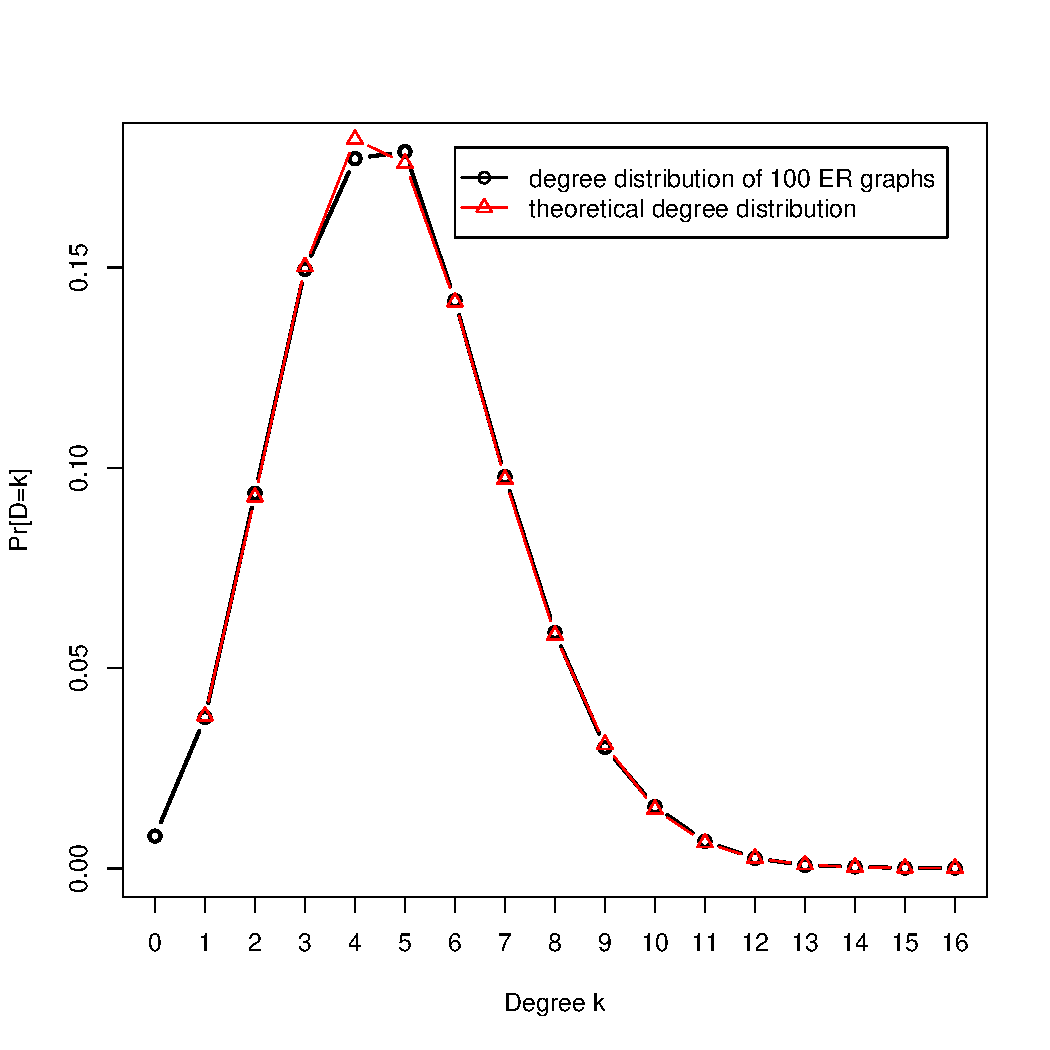
\includegraphics[width=0.9\textwidth]{er_degree_distribution}
  \caption{Comparison of the degree distribution of 100 ER instances
    and the theoretical degree distribution, where $Pr[D=k] =
    \binom{N-1}{k}p^k(1-p)^{N-1-k}=\binom{378}{k}0.013^k\cdot0.987^{378-k}$.}
\end{figure}


\subsection*{10)}
Average of the metrics over the 100 ER random networks:
\begin{itemize}
 \item Number of nodes $N$: 379
 \item Number of links $L$: 914.33
 \item Link density $p$: 0.012764
 \item Average degree $E[D]$: 4.824960
 \item Degree variance $Var[D]$: 4.774007
 \item Clustering coefficient: 0.012574
 \item Assortativity: -0.003513
 \item Average hopcount $E[H]$: 3.928829
 \item Spectral radius $\lambda_1$: 6.006430
 \item Algebraic connectivity $\mu_{N-1}$: 0.025853
 \item Diameter $H_{max}$: 7.980000
\end{itemize}

\subsection*{11)}


\begin{table}[H]
  \centering
  \begin{tabular}{lr}
    \toprule
  Network    & $E[n_{R_\infty}]$ \\
    \midrule
    $G$      &                   \\
    $G_N$    &                   \\
    100 $ER$ &                   \\
\bottomrule
  \end{tabular}
  \caption{Average number ($E[n_{R_\infty}]$) of resistant nodes in
    the steady state for the different network models.}
\end{table}

% Comparison of E_inf


% My observation


% Possible reasons for my observation


% 
A final conclusion which network facilitates information propagation
better is still difficult.  We have a feeling of which network is
better suited for information propagation.  However, there are still
limitations: for example the speed of information propagation. We
know, how many nodes are infected in the $E[n_{R_\infty}]$ state, but
not how fast that occured.

\begin{table}[H]
  \centering
  \begin{tabular}{r|rrr}
    \toprule
Metric      & $G$   & $G_N$ & 100 ER \\
\midrule
$N$         & 379   & 379   & 379    \\
$L$         & 914   & 914   & 914.33 \\
$p$         & 0.013 & 0.013 & 0.013  \\
$E[D]$      & 4.82  & 4.82  & 4.82   \\
$Var[D]$    & 15.46 & 15.46 & 4.77   \\
$C$         & 0.17  & 0.80  & 0.01  \\
$\rho_D$    & -0.30 & -0.08 & 0.00   \\
$E[H]$      & 3.75  & 6.04  & 3.93   \\
$\lambda_1$ & 7.44  & 10.38 & 6.01   \\
$\mu_{N-1}$ & 0.40  & 0.015 & 0.026  \\
$H_{max}$   & 7     & 17    & 7.98   \\
\bottomrule
  \end{tabular}
  \caption{Comparison of all metrics}
\end{table}

\end{document}
